% \begin{document}

\usetikzlibrary{arrows.meta} % For double arrows

\chapter{Decentralized Database}

In the era of big data today, localized instances of relational databases is no
longer enough to hold the volume of data for today's requirements. Distributed
key-value stores have been of a key area of interest in the past few decades. 
Offering such as DynamoDB, Cassandra, and Azure Cloud are a few examples of what
industry leaders are offering to address the data problem.\\

A cluster of nodes collectively offers service provided by a distributed key-value store. The nodes independently restart, update, crash, join, or leave 
the cluster, while the service remains uninterrupted (though with possibly
reduced service). As the user base scales, the service must scale accordingly.\\

Two of the key design principles in distributed data are partition and
replication.\\

A replica group (RG) is a group of nodes that maintain the same set of data.
Nodes in an RG often span multiple availability zones (AZ) to maximize uptime.
In case of a regional value that wipes out an entire AZ, the other nodes in the
RG can still maintain the service albeit at reduced QoS. The nodes in the RG are
kept in sync using consensus protocols such as Raft. A write is only
completed once it has been recorded by the
majority of nodes in the RG.

Partition is a way to split the key space into slices. When the key space is
partitioned, an RG is only responsible for a slice of the key space. Bandwidth
demand is also amortized across all RGs. Partition is typically done using 
consistent hashing. Different from traditional hashing, consistent hashing
minimizes data movement when nodes join and leave the clusters. Consistent
hashing will be covered in detail in a later part of the chapter.\\

Some of the early distributed database design requires a centralized server for
meta management (eg. ZooKeeper). In this chapter, we will specify a fully
decentralized key-value store. To simplify the specification, we will assume 
each node itself is a functioning RG with associated reliability property (this
is considered a solved problem with Raft). This chapter will focus on system
behavior correctness as RGs join or leave the cluster and associated data
migration.

\section{Consistent Hashing}

Before we dive into design details, we must first describe consistent hashing.
With a traditional hashing algorithm, changing the size of the hash space
requires data movement of the entire cluster. This is very undesirable.
Consistent hashing was introduced to minimize data movement, where movement is
only required when adding or removing nodes in the affected range. 

In consistent hashing, the hash space is assumed to be a ring, where the largest
hash value plus one wraps around to the hash of 0. Servers in a consistent
hashing cluster take up different ranges in the ring. For a given request, the
client where the request lands by hashing the request first, then walks the ring
clockwise until it finds a server. \\ 

Assume the following example:

\begin{center}
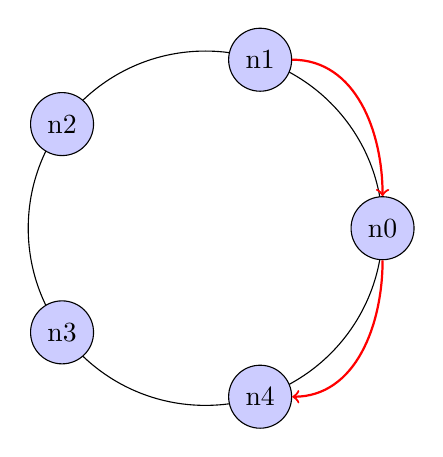
\begin{tikzpicture}[scale=1.5]

    \draw (0,0) circle (1.5cm);

    Draw the nodes on the circle with updated labels
    \foreach \angle/\label in {0/n0, 72/n1, 144/n2, 216/n3, 288/n4} {
        \node[draw, circle, fill=blue!20, minimum size=8mm] at (\angle:1.5cm) (\label) {\label};
    }

    \draw[->, thick, red] (n1) to[out=0, in=90] (n0); % 2 -> 1
    \draw[->, thick, red] (n0) to[out=270, in=0] (n4); % 1 -> 5

\end{tikzpicture}
\end{center}

If the request lands between n1 (exclusive) and n0 (inclusive), the request will
be processed by n0. Similarly, if the request lands between n0 (exclusive) and
n4 (inclusive), the request is to be processed by n4.\\

Assume a case where n4 goes offline: 

\begin{center}
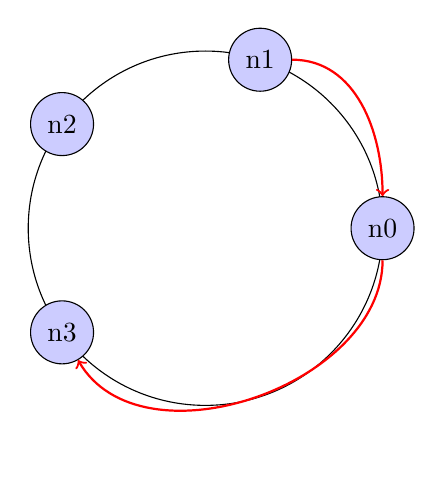
\begin{tikzpicture}[scale=1.5]

    \draw (0,0) circle (1.5cm);

    % Draw the nodes on the circle with updated labels
    \foreach \angle/\label in {0/n0, 72/n1, 144/n2, 216/n3} {
        \node[draw, circle, fill=blue!20, minimum size=8mm] at (\angle:1.5cm) (\label) {\label};
    }

    \draw[->, thick, red] (n1) to[out=0, in=90] (n0); % 2 -> 1
    \draw[->, thick, red] (n0) to[out=270, in=300] (n3); % 1 -> 5

\end{tikzpicture}
\end{center}

In such a case, requests previously processed by n4 will land on n3 instead.
Similarly, if a new node n5 is added:

\begin{center}
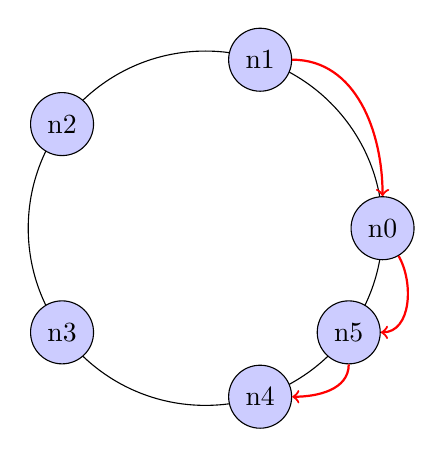
\begin{tikzpicture}[scale=1.5]

    % Draw the circle
    \draw (0,0) circle (1.5cm);

    % Draw the nodes on the circle with updated labels
    \foreach \angle/\label in {0/n0, 72/n1, 144/n2, 216/n3, 288/n4, 324/n5} {
        \node[draw, circle, fill=blue!20, minimum size=8mm] at (\angle:1.5cm) (\label) {\label};
    }

    % Draw arrows
    \draw[->, thick, red] (n1) to[out=0, in=90] (n0); % n1 -> n0
    \draw[->, thick, red] (n0) to[out=300, in=0] (n5); % n0 -> n4
    \draw[->, thick, red] (n5) to[out=270, in=0] (n4); % n0 -> n4

\end{tikzpicture}
\end{center}

Part of what n4 used to service will now be serviced by n5.

\section{Gossip Protocol}

Without a centralized metadata controller, the nodes learn about their peers using
the gossip protocol. As a new RG enters the cluster, the design relies on gossip
protocol to spread the information. This is a critical part of the design as
will be described later.

\section{Design}

In our design, an RG can be in one of the following states: Offline, Joining,
Online, Leaving. The service starts with a single RG responsible for the entire
hash space. Since this is the epoch RG, it directly transitions into an Online
state and can claim any token on the ring. For simplicity, epoch RG always
claims token 0.\\

The design assumes node failure handling is handled within the RG, the
specification will not model RG crash or restart. 

\subsection{Offline}

RG is offline, with no impact on the cluster.

\subsection{Joining}

By definition, the goal of adding an RG U into the cluster is to reduce the load
on another RG V. Since RG U is a new member of the cluster, it may not have the
latest cluster topology. Once RG U announces its presence via a gossip protocol,
it waits for RG V to reach out.\\

When RG V realizes a new RG can share its burden, RG V will coordinate with RG U
to migrate a subset of its data to RG U (the subset RG U will be responsible
for). Once data migration is completed: RG U transitions to the Online state and
starts servicing requests in its range, while RG V rejects requests to the range
RG U has taken over. This range update is also reflected in both RG U and V's
local ring cache and communicated during the next round of gossip protocol.

\subsection{Online}

RG is \textit{Online} and responds to and records requests in its hash range. 

\subsection{Leaving}

Symmetrically, when an RG U is leaving the cluster, an RG V needs to take over the
range and data RG U is currently responsible for. Similarly to join, RG U 
announced its intent to leave and wait for RG V to reach out and coordinate the
handoff. \\

Note when RG U is still waiting or in the middle of hand-off, it is still
\textit{Online} and must respond to request, until RV V fully takes over.

\section{Specification}

\textit{Init} is defined below:\\

\begin{tla}
offline == [k \in RGState |-> 
            IF k = "version" THEN 0 
            ELSE IF k = "token" THEN -1
            ELSE IF k = "state" THEN "offline"
            ELSE "unused"]
seed == [k \in RGState |-> 
            IF k = "version" THEN 1 
            ELSE IF k = "token" THEN 0
            ELSE IF k = "state" THEN "online"
            ELSE "unused"]
Init ==
    /\ local_ring = [i \in RGs |-> 
                        [j \in RGs |-> 
                            IF i = SeedRG /\ j = SeedRG
                            THEN seed
                            ELSE offline ]] 
    /\ local_kv = [i \in RGs |-> {}]
    /\ debug_kv = {}
    /\ debug = {}
\end{tla}
\begin{tlatex}
\@x{ offline \.{\defeq} [ k \.{\in} RGState \.{\mapsto}}%
\@x{ {\IF} k \.{=}\@w{version} \.{\THEN} 0}%
\@x{ \.{\ELSE} {\IF} k \.{=}\@w{token} \.{\THEN} \.{-} 1}%
\@x{ \.{\ELSE} {\IF} k \.{=}\@w{state} \.{\THEN}\@w{offline}}%
\@x{ \.{\ELSE}\@w{unused} ]}%
\@x{ seed \.{\defeq} [ k \.{\in} RGState \.{\mapsto}}%
\@x{\@s{4.1} {\IF} k \.{=}\@w{version} \.{\THEN} 1}%
\@x{\@s{4.1} \.{\ELSE} {\IF} k \.{=}\@w{token} \.{\THEN} 0}%
\@x{\@s{4.1} \.{\ELSE} {\IF} k \.{=}\@w{state} \.{\THEN}\@w{online}}%
\@x{\@s{4.1} \.{\ELSE}\@w{unused} ]}%
\@x{ Init \.{\defeq}}%
\@x{\@s{16.4} \.{\land} local\_ring \.{=} [ i \.{\in} RGs \.{\mapsto}}%
\@x{\@s{20.5} [ j \.{\in} RGs \.{\mapsto}}%
\@x{\@s{24.6} {\IF} i \.{=} SeedRG \.{\land} j \.{=} SeedRG}%
\@x{\@s{24.6} \.{\THEN} seed}%
\@x{\@s{24.6} \.{\ELSE} offline ] ]}%
\@x{\@s{16.4} \.{\land} local\_kv \.{=} [ i \.{\in} RGs \.{\mapsto} \{ \} ]}%
\@x{\@s{16.4} \.{\land} debug\_kv \.{=} \{ \}}%
\@x{\@s{16.4} \.{\land} debug \.{=} \{ \}}%
\end{tlatex}
\\

Since RGs operate independently, each RG maintains its view of the ring. This is
tracked by \textit{local\_ring}. The cluster is initialized with a single RG
\textit{SeedRG} with \textit{version} set to 1, \textit{state} set to online, and
claims \textit{token} 0 on the ring.\\

\textit{local\_kv} represents the per RG KV store. \textit{debug\_kv} records
what the client has written, this is used to verify the consistency of the
distributed database. Finally, a \textit{debug} variable is used to hold a token
in a failure trace.\\

The core set of actions permitted by \textit{Spec} is defined below:\\
\begin{tla}
Next ==
    \/ \E u, v \in RGs:
        /\ Gossip(u, v)
    \/ \E u \in RGs:
        \/ Join(u) 
        \/ JoinMigrate(u)
        \/ Leave(u)
        \/ LeaveMigrate(u)
    \/ \E u \in RGs:
        /\ \E k \in KeySpace:
            /\ k \notin debug_kv
            /\ Write(u, k)
\end{tla}
\begin{tlatex}
\@x{ Next \.{\defeq}}%
\@x{\@s{16.4} \.{\lor} \E\, u ,\, v \.{\in} RGs \.{:}}%
\@x{\@s{20.5} \.{\land} Gossip ( u ,\, v )}%
\@x{\@s{16.4} \.{\lor} \E\, u \.{\in} RGs \.{:}}%
\@x{\@s{20.5} \.{\lor} Join ( u )}%
\@x{\@s{20.5} \.{\lor} JoinMigrate ( u )}%
\@x{\@s{20.5} \.{\lor} Leave ( u )}%
\@x{\@s{20.5} \.{\lor} LeaveMigrate ( u )}%
\@x{\@s{16.4} \.{\lor} \E\, u \.{\in} RGs \.{:}}%
\@x{\@s{20.5} \.{\land} \E\, k \.{\in} KeySpace \.{:}}%
\@x{\@s{24.6} \.{\land} k \.{\notin} debug\_kv}%
\@x{\@s{24.6} \.{\land} Write ( u ,\, k )}%
\end{tlatex}
\\

A RG can \textit{Join} or \textit{Leave} the cluster. However, both are graceful
operations requiring coordination of other nodes from the cluster. To completelyjoin or leave, another RG has to either offload or take over the range of thejoining or leaving RG. This is described by \textit{JoinMigrate} and
\textit{LeaveMigrate}. Any pair of nodes can \textit{Gossip} to share their
understanding of the current cluster state. Finally, a client can \textit{Write}
to the database by sending a request to an RG.\\

Let us take a look at the definition for \textit{Join}:\\
\begin{tla}
ClaimedToken == 
    LET 
        not_offline == {v \in RGs: local_ring[v][v]["state"] # StateOffline}
    IN 
        {local_ring[k][k]["token"]: k \in not_offline}

Join(u) == 
    LET 
        key == CHOOSE any \in KeySpace \ ClaimedToken: TRUE
    IN 
        \* Only ever one node joining at a time
        /\ local_ring[u][u]["state"] = StateOffline
        /\ local_ring' = [local_ring EXCEPT ![u] 
                            = [local_ring[u] EXCEPT ![u]
                                = [k \in RGState |-> 
                                    IF k = "version" THEN local_ring[u][u][k] + 1
                                    ELSE IF k = "token" THEN key
                                    ELSE IF k = "state" THEN StatePrepare
                                    ELSE "unused"]]]
        /\ UNCHANGED <<local_kv, debug_kv, debug>>
\end{tla}
\begin{tlatex}
\@x{ ClaimedToken \.{\defeq}}%
\@x{\@s{16.4} \.{\LET}}%
 \@x{\@s{32.8} not\_offline \.{\defeq} \{ v \.{\in} RGs \.{:} local\_ring [ v
 ] [ v ] [\@w{state} ] \.{\neq} StateOffline \}}%
\@x{\@s{16.4} \.{\IN}}%
 \@x{\@s{32.8} \{ local\_ring [ k ] [ k ] [\@w{token} ] \.{:} k \.{\in}
 not\_offline \}}%
\@pvspace{8.0pt}%
\@x{ Join ( u ) \.{\defeq}}%
\@x{ \.{\LET}}%
 \@x{\@s{16.4} key \.{\defeq} {\CHOOSE} any \.{\in} KeySpace
 \.{\,\backslash\,} ClaimedToken \.{:} {\TRUE}}%
\@x{ \.{\IN}}%
\@x{\@s{16.4}}%
\@y{%
  Only ever one node joining at a time
}%
\@xx{}%
 \@x{\@s{16.4} \.{\land} local\_ring [ u ] [ u ] [\@w{state} ] \.{=}
 StateOffline}%
 \@x{\@s{16.4} \.{\land} local\_ring \.{'} \.{=} [ local\_ring {\EXCEPT}
 {\bang} [ u ]}%
\@x{\@s{24.59} \.{=} [ local\_ring [ u ] {\EXCEPT} {\bang} [ u ]}%
\@x{\@s{28.69} \.{=} [ k \.{\in} RGState \.{\mapsto}}%
 \@x{\@s{32.8} {\IF} k \.{=}\@w{version} \.{\THEN} local\_ring [ u ] [ u ] [ k
 ] \.{+} 1}%
\@x{\@s{32.8} \.{\ELSE} {\IF} k \.{=}\@w{token} \.{\THEN} key}%
\@x{\@s{32.8} \.{\ELSE} {\IF} k \.{=}\@w{state} \.{\THEN} StatePrepare}%
\@x{\@s{32.8} \.{\ELSE}\@w{unused} ] ] ]}%
 \@x{\@s{16.4} \.{\land} {\UNCHANGED} {\langle} local\_kv ,\, debug\_kv ,\,
 debug {\rangle}}%
\end{tlatex}
\\

A RG can only join the cluster if it is currently \textit{Offline}. To join the
cluster, the RG must claim an unclaimed token, enter \textit{Joining} state, and
announces its intent via \textit{Gossip}.\\

The design has taken a shortcut to claim an unclaimed token. In a production
implementation, a newly joined RG will not know which token is unclaimed. Since
the design relies on another RG to \textit{admit} the new RG into the cluster,
in the case of a collision the admitting RG can simply ask the RG that wishes to
join to pick a different token and restart the process. Practically, the hash
space is large enough that collision is unlikely.\\

The following describes \textit{JoinMigrate}:\\
\begin{tla}
RECURSIVE FindPrevToken(_, _)
FindPrevToken(key, ring) ==
    LET 
        condition(v) == ring[v]["state"] # StateOffline 
                    /\ ring[v]["token"] = key
        exists == \E v \in DOMAIN ring: condition(v)
        owner == CHOOSE only \in DOMAIN ring: condition(only)
    IN 
        IF exists THEN
            owner
        ELSE 
            FindPrevToken((key + N - 1) \% N, ring)

JoinMigrate(u) == 
    LET 
        \* previous token
        v == FindPrevToken((local_ring[u][u]["token"] + N - 1) % N, 
                            local_ring[u])
        all_keys == local_kv[u]
        all_online_tokens == AllOnlineTokens(u)
        v_token == local_ring[u][v]["token"]
        v_data == DataSet(v_token, all_online_tokens, all_keys)
        updated == [k \in RGState |-> 
                            IF k = "version" THEN local_ring[u][v]["version"] + 1
                            ELSE IF k = "token" THEN local_ring[u][v]["token"]
                            ELSE IF k = "state" THEN StateOnline
                            ELSE "unused"]
        merged == Merge(u, v)
        local_ring_u == [merged EXCEPT ![u] 
                            = [merged[u] EXCEPT ![v] = updated]]
        local_ring_uv == [local_ring_u EXCEPT ![v] 
                            = [local_ring_u[v] EXCEPT ![v] = updated]]
    IN 
        /\ Cardinality(AllTokens(u)) >= 2
        /\ local_ring[u][u]["state"] = StateOnline
        /\ local_ring[u][v]["state"] = StatePrepare
        /\ Cardinality(all_keys) # 0
        /\ IF v_data # {} THEN 
                /\ local_ring' = local_ring_uv
                /\ local_kv' = [k \in RGs |-> 
                                IF k = u THEN local_kv[k] \ v_data
                                ELSE IF k = v THEN local_kv[k] \cup v_data
                                ELSE local_kv[k]]
            ELSE 
                UNCHANGED <<local_ring, local_kv>>
        /\ UNCHANGED <<debug_kv, debug>>
\end{tla}
\begin{tlatex}
\@x{ {\RECURSIVE} FindPrevToken ( \_ ,\, \_ )}%
\@x{ FindPrevToken ( key ,\, ring ) \.{\defeq}}%
\@x{\@s{16.4} \.{\LET}}%
 \@x{\@s{32.8} condition ( v ) \.{\defeq} ring [ v ] [\@w{state} ] \.{\neq}
 StateOffline}%
\@x{\@s{36.89} \.{\land} ring [ v ] [\@w{token} ] \.{=} key}%
 \@x{\@s{32.8} exists \.{\defeq} \E\, v \.{\in} {\DOMAIN} ring \.{:} condition
 ( v )}%
 \@x{\@s{32.8} owner \.{\defeq} {\CHOOSE} only \.{\in} {\DOMAIN} ring \.{:}
 condition ( only )}%
\@x{\@s{16.4} \.{\IN}}%
\@x{\@s{32.8} {\IF} exists \.{\THEN}}%
\@x{\@s{36.89} owner}%
\@x{\@s{32.8} \.{\ELSE}}%
 \@x{\@s{49.19} FindPrevToken ( ( key \.{+} N \.{-} 1 ) \.{\,\backslash\,}
 \.{\%} N ,\, ring )}%
\@pvspace{8.0pt}%
\@x{ JoinMigrate ( u ) \.{\defeq}}%
\@x{\@s{16.4} \.{\LET}}%
\@x{\@s{32.8}}%
\@y{%
  previous token
}%
\@xx{}%
 \@x{\@s{32.8} v \.{\defeq} FindPrevToken ( ( local\_ring [ u ] [ u ]
 [\@w{token} ] \.{+} N \.{-} 1 ) \.{\%} N ,\,}%
\@x{\@s{32.8} local\_ring [ u ] )}%
\@x{\@s{32.8} all\_keys \.{\defeq} local\_kv [ u ]}%
\@x{\@s{32.8} all\_online\_tokens \.{\defeq} AllOnlineTokens ( u )}%
\@x{\@s{32.8} v\_token \.{\defeq} local\_ring [ u ] [ v ] [\@w{token} ]}%
 \@x{\@s{32.8} v\_data \.{\defeq} DataSet ( v\_token ,\, all\_online\_tokens
 ,\, all\_keys )}%
\@x{\@s{32.8} updated \.{\defeq} [ k \.{\in} RGState \.{\mapsto}}%
 \@x{\@s{41.0} {\IF} k \.{=}\@w{version} \.{\THEN} local\_ring [ u ] [ v ]
 [\@w{version} ] \.{+} 1}%
 \@x{\@s{41.0} \.{\ELSE} {\IF} k \.{=}\@w{token} \.{\THEN} local\_ring [ u ] [
 v ] [\@w{token} ]}%
\@x{\@s{41.0} \.{\ELSE} {\IF} k \.{=}\@w{state} \.{\THEN} StateOnline}%
\@x{\@s{41.0} \.{\ELSE}\@w{unused} ]}%
\@x{\@s{32.8} merged \.{\defeq} Merge ( u ,\, v )}%
\@x{\@s{32.8} local\_ring\_u \.{\defeq} [ merged {\EXCEPT} {\bang} [ u ]}%
\@x{\@s{45.1} \.{=} [ merged [ u ] {\EXCEPT} {\bang} [ v ] \.{=} updated ] ]}%
 \@x{\@s{32.8} local\_ring\_uv \.{\defeq} [ local\_ring\_u {\EXCEPT} {\bang} [
 v ]}%
 \@x{\@s{41.0} \.{=} [ local\_ring\_u [ v ] {\EXCEPT} {\bang} [ v ] \.{=}
 updated ] ]}%
\@x{\@s{16.4} \.{\IN}}%
\@x{\@s{32.8} \.{\land} Cardinality ( AllTokens ( u ) ) \.{\geq} 2}%
 \@x{\@s{32.8} \.{\land} local\_ring [ u ] [ u ] [\@w{state} ] \.{=}
 StateOnline}%
 \@x{\@s{32.8} \.{\land} local\_ring [ u ] [ v ] [\@w{state} ] \.{=}
 StatePrepare}%
\@x{\@s{32.8} \.{\land} Cardinality ( all\_keys ) \.{\neq} 0}%
\@x{\@s{32.8} \.{\land} {\IF} v\_data \.{\neq} \{ \} \.{\THEN}}%
\@x{\@s{41.0} \.{\land} local\_ring \.{'} \.{=} local\_ring\_uv}%
\@x{\@s{41.0} \.{\land} local\_kv \.{'} \.{=} [ k \.{\in} RGs \.{\mapsto}}%
 \@x{\@s{41.0} {\IF} k \.{=} u \.{\THEN} local\_kv [ k ] \.{\,\backslash\,}
 v\_data}%
 \@x{\@s{41.0} \.{\ELSE} {\IF} k \.{=} v \.{\THEN} local\_kv [ k ] \.{\cup}
 v\_data}%
\@x{\@s{41.0} \.{\ELSE} local\_kv [ k ] ]}%
\@x{\@s{36.89} \.{\ELSE}}%
\@x{\@s{53.29} {\UNCHANGED} {\langle} local\_ring ,\, local\_kv {\rangle}}%
\@x{\@s{32.8} \.{\land} {\UNCHANGED} {\langle} debug\_kv ,\, debug {\rangle}}%
\end{tlatex}
\\

A RG U walks its local ring counter-clockwise to find the first neighboring RG
V. If RG V is in \textit{Joining} state, this allows RG U to offload part of
its range to RG V and admit RG V into the cluster. This coordination also
includes data migration, since some of the keys RG U has will be owned by RG V
as well. At the end of the process, both RG U and V update their local ring cache of
each other's state and propagate that in subsequent rounds of \textit{Gossip}.\\

In a practical implementation, the data migration process might take a while.
The RGs maintains merkle-trees for its data and uses that to determine
migration status. Once data migration completes, the range switchover is atomic. 
RG U stops servicing requests to the range RG V has taken over and redirects 
the requests to RG V either explicitly or implicitly via gossip protocol.\\

The following defines \textit{Leave}:\\

\begin{tla}
Leave(u) == 
    LET 
        updated == [k \in RGState |-> 
                     IF k = "version" THEN local_ring[u][u][k] + 1
                     ELSE IF k = "token" THEN local_ring[u][u][k]
                     ELSE IF k = "state" THEN StateExit
                     ELSE "unused"]
    IN 
        \* can only leave if we are already online 
        /\ local_ring[u][u]["state"] = StateOnline
        \* can only leave if there's at least another server to migrate data to
        /\ Cardinality(AllOnlineTokens(u)) >= 2
        /\ local_ring' = [local_ring EXCEPT ![u] 
                            = [local_ring[u] EXCEPT ![u]
                                = updated]] 
        /\ UNCHANGED <<local_kv, debug_kv, debug>>
\end{tla}
\begin{tlatex}
\@x{ Leave ( u ) \.{\defeq}}%
\@x{\@s{16.4} \.{\LET}}%
\@x{\@s{32.8} updated \.{\defeq} [ k \.{\in} RGState \.{\mapsto}}%
 \@x{\@s{36.89} {\IF} k \.{=}\@w{version} \.{\THEN} local\_ring [ u ] [ u ] [
 k ] \.{+} 1}%
 \@x{\@s{36.89} \.{\ELSE} {\IF} k \.{=}\@w{token} \.{\THEN} local\_ring [ u ]
 [ u ] [ k ]}%
\@x{\@s{36.89} \.{\ELSE} {\IF} k \.{=}\@w{state} \.{\THEN} StateExit}%
\@x{\@s{36.89} \.{\ELSE}\@w{unused} ]}%
\@x{\@s{16.4} \.{\IN}}%
\@x{\@s{32.8}}%
\@y{%
  can only leave if we are already online 
}%
\@xx{}%
 \@x{\@s{32.8} \.{\land} local\_ring [ u ] [ u ] [\@w{state} ] \.{=}
 StateOnline}%
\@x{\@s{32.8}}%
\@y{%
  can only leave if there's at least another server to migrate data to
}%
\@xx{}%
\@x{\@s{32.8} \.{\land} Cardinality ( AllOnlineTokens ( u ) ) \.{\geq} 2}%
 \@x{\@s{32.8} \.{\land} local\_ring \.{'} \.{=} [ local\_ring {\EXCEPT}
 {\bang} [ u ]}%
\@x{\@s{41.0} \.{=} [ local\_ring [ u ] {\EXCEPT} {\bang} [ u ]}%
\@x{\@s{45.1} \.{=} updated ] ]}%
 \@x{\@s{32.8} \.{\land} {\UNCHANGED} {\langle} local\_kv ,\, debug\_kv ,\,
 debug {\rangle}}%
\end{tlatex}
\\

Similar to \textit{Join}, a RG can leave if it is \textit{Online}, and not the
only RG in the cluster.\\

Correspondingly, the following defines \textit{LeaveMigrate}:\\
\begin{tla}
LeaveMigrate(u) == 
    LET 
        token == (local_ring[u][u]["token"] + N - 1) % N
        v == FindPrevToken(token, local_ring[u])
        data == local_kv[u] 

        updated == [k \in RGState |-> 
                            IF k = "version" THEN local_ring[u][v]["version"] + 1
                            ELSE IF k = "token" THEN local_ring[u][v]["token"]
                            ELSE IF k = "state" THEN StateOffline
                            ELSE "unused"]
        merged == Merge(u, v)
        local_ring_u == [merged EXCEPT ![u] 
                            = [merged[u] EXCEPT ![v] = updated]]
        local_ring_uv == [local_ring_u EXCEPT ![v] 
                            = [local_ring_u[v] EXCEPT ![v] = updated]]
    IN 
        \* copying from v to u
        /\ local_ring[u][u]["state"] = StateOnline
        /\ local_ring[u][v]["state"] = StateExit
        \* update version 
        /\ local_ring' = local_ring_uv
        \* migrate data
        /\ local_kv' = [k \in RGs |-> 
                        IF k = v THEN {} 
                        ELSE IF k = u THEN local_kv[v] \cup local_kv[u] 
                        ELSE local_kv[k]]
        /\ UNCHANGED <<debug_kv, debug>>
\end{tla}
\begin{tlatex}
\@x{ LeaveMigrate ( u ) \.{\defeq}}%
\@x{\@s{16.4} \.{\LET}}%
 \@x{\@s{32.8} token \.{\defeq} ( local\_ring [ u ] [ u ] [\@w{token} ] \.{+}
 N \.{-} 1 ) \.{\%} N}%
\@x{\@s{32.8} v \.{\defeq} FindPrevToken ( token ,\, local\_ring [ u ] )}%
\@x{\@s{32.8} data \.{\defeq} local\_kv [ u ]}%
\@pvspace{8.0pt}%
\@x{\@s{32.8} updated \.{\defeq} [ k \.{\in} RGState \.{\mapsto}}%
 \@x{\@s{41.0} {\IF} k \.{=}\@w{version} \.{\THEN} local\_ring [ u ] [ v ]
 [\@w{version} ] \.{+} 1}%
 \@x{\@s{41.0} \.{\ELSE} {\IF} k \.{=}\@w{token} \.{\THEN} local\_ring [ u ] [
 v ] [\@w{token} ]}%
\@x{\@s{41.0} \.{\ELSE} {\IF} k \.{=}\@w{state} \.{\THEN} StateOffline}%
\@x{\@s{41.0} \.{\ELSE}\@w{unused} ]}%
\@x{\@s{32.8} merged \.{\defeq} Merge ( u ,\, v )}%
\@x{\@s{32.8} local\_ring\_u \.{\defeq} [ merged {\EXCEPT} {\bang} [ u ]}%
\@x{\@s{45.1} \.{=} [ merged [ u ] {\EXCEPT} {\bang} [ v ] \.{=} updated ] ]}%
 \@x{\@s{32.8} local\_ring\_uv \.{\defeq} [ local\_ring\_u {\EXCEPT} {\bang} [
 v ]}%
 \@x{\@s{41.0} \.{=} [ local\_ring\_u [ v ] {\EXCEPT} {\bang} [ v ] \.{=}
 updated ] ]}%
\@x{\@s{16.4} \.{\IN}}%
\@x{\@s{32.8}}%
\@y{%
  copying from v to u
}%
\@xx{}%
 \@x{\@s{32.8} \.{\land} local\_ring [ u ] [ u ] [\@w{state} ] \.{=}
 StateOnline}%
 \@x{\@s{32.8} \.{\land} local\_ring [ u ] [ v ] [\@w{state} ] \.{=}
 StateExit}%
\@x{\@s{32.8}}%
\@y{%
  update version 
}%
\@xx{}%
\@x{\@s{32.8} \.{\land} local\_ring \.{'} \.{=} local\_ring\_uv}%
\@x{\@s{32.8}}%
\@y{%
  migrate data
}%
\@xx{}%
\@x{\@s{32.8} \.{\land} local\_kv \.{'} \.{=} [ k \.{\in} RGs \.{\mapsto}}%
\@x{\@s{32.8} {\IF} k \.{=} v \.{\THEN} \{ \}}%
 \@x{\@s{32.8} \.{\ELSE} {\IF} k \.{=} u \.{\THEN} local\_kv [ v ] \.{\cup}
 local\_kv [ u ]}%
\@x{\@s{32.8} \.{\ELSE} local\_kv [ k ] ]}%
\@x{\@s{32.8} \.{\land} {\UNCHANGED} {\langle} debug\_kv ,\, debug {\rangle}}%
\end{tlatex}
\\

Similar to \textit{JoinMigrate}: when RG U finds out its neighbor RV V intends
to leave the cluster, it coordinates with RG V to migrate its data and range.\\

\textit{Gossip} is defined below:\\
\begin{tla}
Merge(u, v) == 
    LET 
        updated(w) ==   IF local_ring[u][w]["version"] 
                            < local_ring[v][w]["version"] THEN 
                            local_ring[v][w]
                        ELSE 
                            local_ring[u][w]
    IN 
        [k \in RGs |-> IF k = u \/ k = v 
                         THEN [w \in RGs |-> updated(w)]
                         ELSE local_ring[k]]

Gossip(u, v) == 
    /\ local_ring[u][u]["state"] # StateOffline
    /\ local_ring[v][v]["state"] # StateOffline
    /\ local_ring' = Merge(u, v)
    /\ UNCHANGED <<local_kv, debug_kv, debug>>
\end{tla}
\begin{tlatex}
\@x{ Merge ( u ,\, v ) \.{\defeq}}%
\@x{\@s{16.4} \.{\LET}}%
 \@x{\@s{32.8} updated ( w ) \.{\defeq}\@s{8.2} {\IF} local\_ring [ u ] [ w ]
 [\@w{version} ]}%
\@x{\@s{45.1} \.{<} local\_ring [ v ] [ w ] [\@w{version} ] \.{\THEN}}%
\@x{\@s{45.1} local\_ring [ v ] [ w ]}%
\@x{\@s{41.0} \.{\ELSE}}%
\@x{\@s{57.4} local\_ring [ u ] [ w ]}%
\@x{\@s{16.4} \.{\IN}}%
\@x{\@s{32.8} [ k \.{\in} RGs \.{\mapsto} {\IF} k \.{=} u \.{\lor} k \.{=} v}%
\@x{\@s{41.0} \.{\THEN} [ w \.{\in} RGs \.{\mapsto} updated ( w ) ]}%
\@x{\@s{41.0} \.{\ELSE} local\_ring [ k ] ]}%
\@pvspace{8.0pt}%
\@x{ Gossip ( u ,\, v ) \.{\defeq}}%
 \@x{\@s{16.4} \.{\land} local\_ring [ u ] [ u ] [\@w{state} ] \.{\neq}
 StateOffline}%
 \@x{\@s{16.4} \.{\land} local\_ring [ v ] [ v ] [\@w{state} ] \.{\neq}
 StateOffline}%
\@x{\@s{16.4} \.{\land} local\_ring \.{'} \.{=} Merge ( u ,\, v )}%
 \@x{\@s{16.4} \.{\land} {\UNCHANGED} {\langle} local\_kv ,\, debug\_kv ,\,
 debug {\rangle}}%
\end{tlatex}
\\

\textit{Gossip} can happen between any pair of nodes as long as they are both 
\textit{not Offline}.\\

Finally, let us take a look at \textit{Write}:\\
\begin{tla}
Write(u, k) == 
    LET 
        owner == FindNextToken(k, local_ring[u])
    IN 
        \* only accept if u is owner
        /\ \/ local_ring[u][u]["state"] = StateOnline
           \/ local_ring[u][u]["state"] = StateExit
        /\ u = owner
        /\ local_kv' = [local_kv EXCEPT ![u] 
                        = local_kv[u] \cup {k}]
        /\ debug_kv' = debug_kv \cup {k}
        /\ UNCHANGED <<local_ring, debug>>
\end{tla}
\begin{tlatex}
\@x{ Write ( u ,\, k ) \.{\defeq}}%
\@x{\@s{16.4} \.{\LET}}%
\@x{\@s{32.8} owner \.{\defeq} FindNextToken ( k ,\, local\_ring [ u ] )}%
\@x{\@s{16.4} \.{\IN}}%
\@x{\@s{32.8}}%
\@y{%
  only accept if u is owner
}%
\@xx{}%
 \@x{\@s{32.8} \.{\land} \.{\lor} local\_ring [ u ] [ u ] [\@w{state} ] \.{=}
 StateOnline}%
\@x{\@s{32.8} \.{\lor} local\_ring [ u ] [ u ] [\@w{state} ] \.{=} StateExit}%
\@x{\@s{32.8} \.{\land} u \.{=} owner}%
 \@x{\@s{32.8} \.{\land} local\_kv \.{'} \.{=} [ local\_kv {\EXCEPT} {\bang} [
 u ]}%
\@x{\@s{32.8} \.{=} local\_kv [ u ] \.{\cup} \{ k \} ]}%
\@x{\@s{32.8} \.{\land} debug\_kv \.{'} \.{=} debug\_kv \.{\cup} \{ k \}}%
 \@x{\@s{32.8} \.{\land} {\UNCHANGED} {\langle} local\_ring ,\, debug
 {\rangle}}%
\end{tlatex}
\\

An RG in \textit{Joining} state cannot accept requests because it has not been
admitted into the cluster. A RG in \textit{Leaving} state must still
accept requests because the hand-off hasn't been completed. The specification 
enforces an RG to only accept requests in its data range. A practical
implementation will include some sort of explicit or implicit redirect.

\section{Safety}

The design assumes RG maintains its own data replication internally. This implies 
data should not be between RGs:\\

\begin{tla}
DataUnique == 
    \A u, v \in RGs:
        /\ u # v => local_kv[u] \intersect local_kv[v] = {}
\end{tla}
\begin{tlatex}
\@x{ DataUnique \.{\defeq}}%
\@x{\@s{16.4} \A\, u ,\, v \.{\in} RGs \.{:}}%
 \@x{\@s{16.4} \.{\land} u \.{\neq} v \.{\implies} local\_kv [ u ] \.{\cap}
 local\_kv [ v ] \.{=} \{ \}}%
\end{tlatex}

Every RG maintains a set of key values in its KV store. We want to confirm all the keys 
in the KV store has not been misplaced:\\

\begin{tla}
TokenLocation == 
    \A u \in RGs:
        \A k \in local_kv[u]: 
            u = FindNextToken(k, local_ring[u])
\end{tla}
\begin{tlatex}
\@x{ TokenLocation \.{\defeq}}%
\@x{\@s{16.4} \A\, u \.{\in} RGs \.{:}}%
\@x{\@s{20.5} \A\, k \.{\in} local\_kv [ u ] \.{:}}%
\@x{\@s{24.6} u \.{=} FindNextToken ( k ,\, local\_ring [ u ] )}%
\end{tlatex}

The union of all the KV stores needs to mirror all the data written:\\

\begin{tla}
KVConsistent == 
    /\ UNION {local_kv[n] : n \in RGs} = debug_kv
\end{tla}
\begin{tlatex}
\@x{ KVConsistent \.{\defeq}}%
 \@x{\@s{16.4} \.{\land} {\UNION} \{ local\_kv [ n ] \.{:} n \.{\in} RGs \}
 \.{=} debug\_kv}%
\end{tlatex}

\section{Liveness}

Omitted for this chapter.

% \end{document}
